% !TEX encoding = UTF-8
% !TEX TS-program = pdflatex
% !TEX root = ../tesi.tex
% !TEX spellcheck = it-IT

%**************************************************************
\chapter{Verifica e validazione}
\label{cap:verifica-validazione}
%**************************************************************

\intro{Breve introduzione al capitolo}\\
Questo capitolo descrive i test effettuati per garantire la qualità del codice prodotto durante l'implementazione di \emph{SkillMatrix} e i risultati di tali verifiche.
%**************************************************************

\section{Test di unità}
L'approccio \emph{Test Driven} garantisce intrinsecamente che ogni unità software sia testata ancora prima della sua implementazione. Ogni unità dovrebbe contenere il quantitativo minimo di codice necessario a far rendere positivo il test ideato e scritto in precedenza.\\
Questo approccio, sebbene all'inizio sia piuttosto insolito ed a prima vista tedioso, risulta invece essere imprescindibile nello sviluppo di applicazioni web, soprattutto utilizzando \emph{framework} JavaScript. AngularJS stesso è stato pensato per scrivere applicazioni facilmente testabili, includendo al suo interno delle librerie create appositamente per il testing.\\
Mi è stato quindi possibile testare ogni componente della logica dell'applicazione, controllando il comportamento delle unità e dei loro metodi. Tramite l'utilizzo di sistemi di automazione, nel mio caso \emph{Karma}, sono riuscito a rendere il processo di testing quanto più automatico possibile ed a calcolare con facilità le metriche base per verificare l'utilità dei test scritti.\\
Tramite il plugin di \emph{coverage} di Karma, ho generato automaticamente tali cifre, suddividendole per:
\begin{itemize}
	\item line coverage;
	\item statement coverage;
	\item branch coverage;
	\item function coverage.
\end{itemize}
Nella figura sottostante, presento i dati in forma tabellare, come vengono visualizzati dall'output del \emph{plugin} \emph{karma-coverage}, installabile facilmente da \gls{npm}.

\begin{figure}[!h] 
    \centering 
    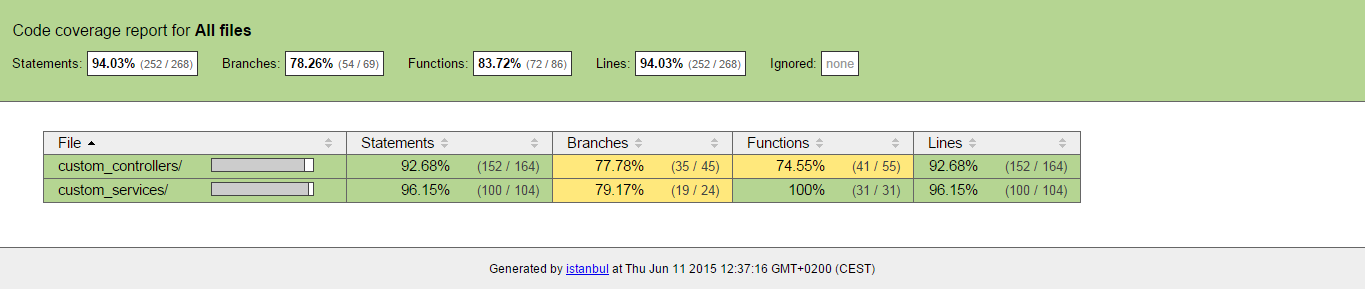
\includegraphics[width=0.9\columnwidth]{coverage/coverage_all} 
    \caption{Metriche di copertura generali nel progetto \emph{SkillMatrix}}
\end{figure}

\begin{figure}[!h] 
    \centering 
    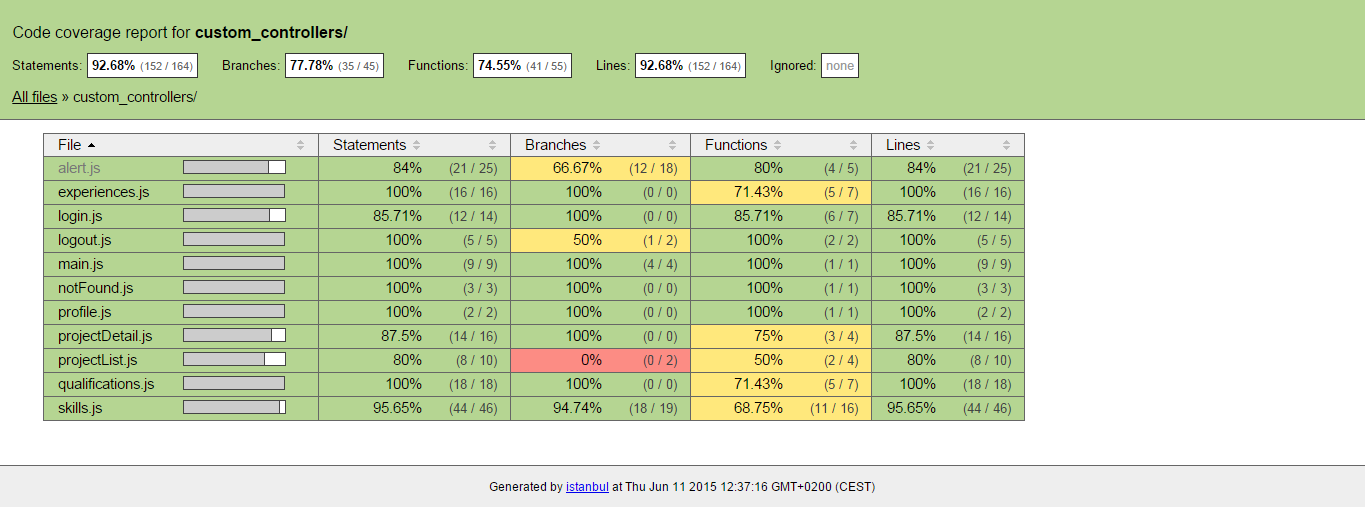
\includegraphics[width=0.9\columnwidth]{coverage/coverage_controllers} 
    \caption{Metriche di copertura dei \emph{controller} nel progetto \emph{SkillMatrix}}
\end{figure}

\begin{figure}[!h] 
    \centering 
    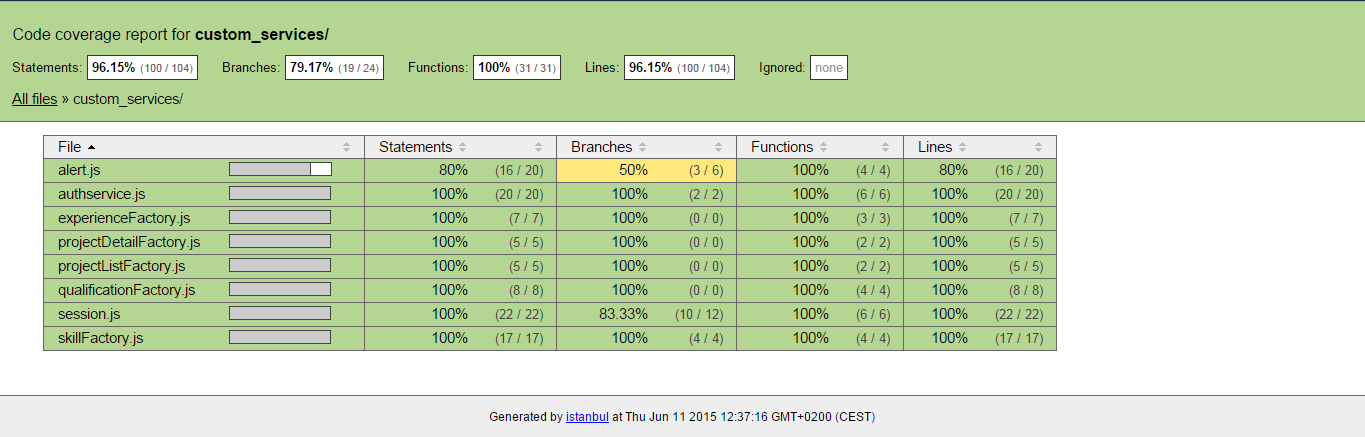
\includegraphics[width=0.9\columnwidth]{coverage/coverage_services} 
    \caption{Metriche di copertura dei servizi nel progetto \emph{SkillMatrix}}
\end{figure}

\subsection{Test di unità di AngularJS}
La scrittura e l'esecuzione dei test nello sviluppo in linguaggio JavaScript è imprescindibile. Su questa base sono nati svariati \emph{framework} di testing, ed AngularJS cerca di semplificare al massimo queste attività. Questo \emph{framework} dispone di diverse direttive utili al fine di simulare il comportamento di componenti esterne, che possono essere anche non ancora state realizzate al tempo della scrittura del test. Infatti, AngularJS comprende anche il pacchetto \emph{angular-mocks}, il quale fornisce tutta una serie di librerie per AngularJS dedicate solamente ai test del \gls{front-end}.\\
All'interno di questo pacchetto vi sono costruttori di \gls{stub} che simulano il comportamento di ogni tipo di componente di AngularJS: dai \emph{controller}, ai servizi, alle singole chiamate verso il \gls{back-end}. Nei singoli test di unità, infatti, è importante testare il comportamento di una componente a seconda dei dati in input, automatizzando il tutto il più possibile.\\
Fra le tante direttive presenti nel pacchetto \emph{angular-mocks}, una delle più utili è di sicuro stata \textbf{\$httpBackend}, la quale simula il comportamento di un \gls{back-end} fittizio, al fine di controllare la struttura ed il contenuto delle chiamate effettuate al \gls{back-end}, senza per forza disporre di un \gls{back-end} e per automatizzare le attività di testing in locale.\\
\textbf{\$httpBackend} agisce in modo da frapporsi tra il \gls{front-end} di AngularJS ed il \gls{back-end}, intercettando le chiamate per analizzarne le richieste; inoltre si può fare in modo di fornire delle risposte definite al \emph{client}, in modo da testare il comportamento dell'unità che si sta verificando. L'intercettazione delle chiamate è selettiva, quindi si può scegliere di filtrare delle richieste di una specifica risorsa \gls{rest} piuttosto che un'altra.
\begin{verbatim}
it('should get project list from server', function() {
  $httpBackend.expectGET('/api/' + APP_VERSION.version + '/users/' + username + '/projects')
    .respond(200, {
      data: {
        projects: [
          {
            projectTitle: 'Smash',
            registered: true
          },
          {
            projectTitle: 'Linko',
            registered: true
          },
          {
            projectTitle: 'SkillMatrix',
            registered: false
          }
        ]
      }
    });
    var responseData = [];
    ProjListFactory.getProjects(username).success(function(data) {
      responseData = data.data.projects;
    });
  $httpBackend.flush();
  expect(responseData.length).toBe(3);
  expect(responseData[0].projectTitle).toBe('Smash');
  expect(responseData[1].registered).toBeTruthy();
  expect(responseData[2].registered).toBeFalsy();
});
\end{verbatim}
Questo frammento di codice testa che i dati di una lista di progetti siano ottenuti e gestiti secondo la formattazione stabilita. Si può notare che la richiesta che viene intercettata è una richiesta \gls{rest} particolare, in quanto si vuole testare una singola funzionalità per volta. Vengono quindi forniti dei dati fittizi in risposta in modo da controllare il comportamento del modulo alla gestione dei dati; il modo in cui questo viene fatto in \emph{Jasmine} è di controllare che le aspettative degli output siano confrontate con i dati attuali all'esecuzione del test, per vedere se entrambi combaciano.

%**************************************************************

\newpage

\section{Test End-To-End}
I test di scenario (o \gls{e2e}) servono a verificare la corretta interazione di uno o più unità software al fine di perseguire una certa azione dell'utente. AngularJS consiglia di utilizzare lo \emph{stack} fornito da \emph{Protractor} e da \emph{Selenium} per automatizzare il processo di testing. Ogni test di scenario automatizza gli input utente in un browser ed analizza gli output ad ogni modifica.\\
Questi test sono molto più laboriosi di un test di unità eseguito con \emph{Karma}, ma sono molto più vicini ad essere dei test di validazione.\\
In questo progetto ho creato un test per ogni tipo di azione utente, dalla semplice consultazione di informazioni del profilo all'inserimento di una nuova \emph{skill} nel sistema. Ogni test avviene automatizzando l'input attraverso la selezione dei vari elementi \gls{html} della pagina a cui fa riferimento il test e gli elementi vengono individuati tramite semplici selettori \gls{css} o \emph{jQuery}.\\

\begin{figure}[!h] 
    \centering 
    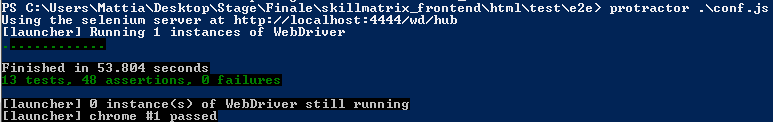
\includegraphics[width=0.9\columnwidth]{e2e} 
    \caption{Grafica da console dell'esecuzione di test \gls{e2e} di Protractor}
\end{figure}

Ogni test è composto di passi ben precisi, ovvero le stesse azioni che compongono l'input utente. Il test quindi deve effettuare gli stessi passi, compresi i singoli click su dei link e l'input di testo quando richiesto. La prossima porzione di codice è il test \gls{e2e} del login, sia errato che corretto, con le proprie \emph{expectations}, ovvero i valori previsti in output.

\begin{verbatim}
'use strict';

describe('SkillMatrix login', function() {

  beforeEach(function() {
    browser.get('base.html');
    browser.waitForAngular();
  });

  it('should have a title', function() {
    expect(browser.getTitle()).toEqual('SkillMatrix');
  });

  it('should appear an error message on wrong login', function() {
    element(by.model('credentials.name')).sendKeys('IKS');
    element(by.model('credentials.password')).sendKeys(2);

    element(by.css('button[type="submit"]')).click();

    expect(element(by.binding('alert.message')).getText()).
        toEqual('I dati di autenticazione sono errati(1)');
  });

  it('should login correctly with right credentials', function() {
    element(by.model('credentials.name')).sendKeys('IKS');
    element(by.model('credentials.password')).sendKeys('pippo');

    element(by.css('button[type="submit"]')).click();

    browser.getLocationAbsUrl().then(function(url) {
        expect(url.split('#')[1]).toBe('/profile');
      });
  });
  
});
\end{verbatim}